\documentclass{report}
\usepackage[utf8]{inputenc}
\usepackage{amsmath,amsthm,amsfonts,amssymb,amscd}
\usepackage[a4paper,hmargin=0.8in,bottom=1.3in]{geometry}
\usepackage{lastpage,enumerate,fancyhdr,mathrsfs,xcolor,graphicx,listings,hyperref,enumitem}
\newcommand*{\algodis}[4]{
    \textbf{#1:} #2\\%name: % key idea
    \textbf{Time:} #3 \\% O(what)
    \textbf{Space:} #4
}
\author{Hardik Rajpal}
\newcommand{\trow}[2]{\hline #1 & #2 \\}
\begin{document}
\definecolor{codegreen}{rgb}{0,0.6,0}
\definecolor{codegray}{rgb}{0.5,0.5,0.5}
\definecolor{codepurple}{rgb}{0.58,0,0.82}
\definecolor{backcolour}{rgb}{0.95,0.95,0.92}

\lstdefinestyle{mystyle}{
    backgroundcolor=\color{backcolour},   
    commentstyle=\color{codegreen},
    keywordstyle=\color{magenta},
    numberstyle=\tiny\color{codegray},
    stringstyle=\color{codepurple},
    basicstyle=\ttfamily\footnotesize,
    breakatwhitespace=false,         
    breaklines=true,                 
    captionpos=b,                    
    keepspaces=true,                 
    numbers=left,                    
    numbersep=5pt,                  
    showspaces=false,                
    showstringspaces=false,
    showtabs=false,                  
    tabsize=2
}

\lstset{style=mystyle,language=C++}
\title{Pre-Placement Grind}
\maketitle
\tableofcontents
\pagebreak
\chapter{Misc.}
\section{Misc. Confirmed Optimizations}
\begin{enumerate}
    \item For maps,
\begin{lstlisting}
    auto iter = m.find(k);
    if(iter!=m.end()){return iter->second;}
    //is much faster than:
    if(m.count(k)){return m[k];}
\end{lstlisting}
    \item Replace sets that check for inclusion by bit operations with an integer if the number elements $<$ 32 for ints and 64 for long longs. 
    \item Pass params by reference where possible.
    \item Instead of a reference parameter, consider using a pointer to that variable stored in a class data member.
    \item Replace data types by smaller data types where possible:
        \begin{itemize}
            \item long long by int
            \item int by char
        \end{itemize} 
    \item Replace fixed-length vectors by array$<$type,fixed-length$>$.
    \item Replace maps by vectors if they are indexed by integers within a fixed range. Ex: the alphabet as indices.
    \item That die roll problem optimization. (Needs to be phrased more mathematically.)
    \item Use of suffix arrays + descending order (or its prefix counterpart) to cut of paths in backtracking.
\end{enumerate}
\section{Binary Representations}
\subsection{Unsigned numbers}
Represent n using k bits $b_{k-1}b_{k-2}...b_0$:
\begin{equation}
n \in \{0,1,...2^{k}-1\}, n = \sum_{i=0}^{k-1}b_i\times2^{i}
\end{equation}
\subsection{1's complement}
Represent n using k bits $b_{k-1}b_{k-2}...b_0$:
\begin{equation}
n \in {-(2^{k-1}-1),...-0,0,1,...2^{k-1}-1}, n = (-1)^{b_{k-1}}(\sum_{i=0}^{k-2} (c_i) \times 2^{i})
\end{equation} 
\begin{itemize}
\item Where if $b_{k-1}==1$, $c_i=1-b_i$, else $c_i=b_i$.
\item It has two representations of zero: 1* and 0*.
\item MSB = 1 $\implies$ n $\leq$ 0, else n $\geq$ 0.
\item Bits to n is equivalent to 
\begin{itemize}
    \item Identify sign based on MSB.
    \item If MSB ==1, flip all bits.
    \item Find the unsigned integer they represent and combine the sign.
\end{itemize}
\item To take one's complement of a number is to find its negative counterpart.
\item It is equivalent to just flipping every bit.
\end{itemize}
\subsection{2's complement}
Represent n using k bits $b_{k-1}b_{k-2}...b_0$:
\begin{equation}
n \in \{2^{k-1}, 2^{k-1}-1, ... -1,0,1,...2^{k-1}-1\}, n = (-1)^{b_{k-1}}\sum_{i=0}^{i=k-1} b_i \times 2^i
\end{equation}
\begin{itemize}
\item To take 2's complement of a number is to flip its bits and add 1 to it.
\item This is equivalent to finding its negative in the 2's complement notation.
\end{itemize}
\section{Modular Arithmetic}
\begin{itemize}
\item a \% b returns the remainder when a is divided by b.
\item $a \% b = a - floor(a/b)*b$.
\item $a \equiv b mod n \iff a\%n == b\% n \iff (a-b) \% n == 0 $
\item The congruence relation modulo n splits integers into\\n residue (equivalence) classe $\{C_i\}_{i=0}^{i=n-1}$:
\begin{equation}
    C_i = {z \| z \% n = i};
\end{equation}
\item Representative of $C_i$ is $r_i \in C_i, 0 \le r_i \le n-1$
\item Operations:
\begin{itemize}
\item $a + b \% m = ((a \% m) + (b \% m)) \% m$
\item $a - b \% m = ((a \% m) - (b \% m)) \% m$
\item $(a*b) \% m = ((a \% m) * (b \% m)) \% m$
\item $(a/b) \% m = ((a \% m) * (b^{-1} \% m)) \% m$
\end{itemize}
\item Note: in c++,  a \% m where a<0 returns -((-a)\%m), which is not equal to the mathematical result of
(m - ((-a) \% m)). 
\item If a < 0, a mod m should be calculated as (m + (a \% m)).
\item Or the following function extends to both negative and positive a's : (m + (a \% m)) \% m.
\item Exponentiation.
\item $a == b \mod m \implies a^e = b^e \mod m.$
\item Note: the converse is NOT true. It results in an algebraic equations with possibly multiple roots.
\item $a^e = a^c \mod n \iff e == c \mod \phi(n)$ and gcd(a,n) == 1.
\item If n is prime, then $a^e = a^{e \mod \phi(n)} \mod n \forall a$  
\item TODO: CRT, problems.
\end{itemize}

\section{Master Theorem for Recurrence}

\begin{equation}
T(n) \le aT(n/b) + cn^d \implies
T(n) \le a^{log_b(n)}T(0) + c.n^d.(\sum_{i=1}^{log_b(n)-1}{\frac{a}{b^d}})
\end{equation}
\begin{equation}
\implies T(n) = 
\begin{cases}
O(n^dlog(n)) & a = b^d \\
O(n^d) & a < b^d \\
O(n^{log_b(a)}) & a > b^d 
\end{cases}    
\end{equation}

\section{Useful In-Built C++ functions}
\begin{enumerate}
\item \texttt{swap()}
\item \texttt{lcm, gcd}
\item \texttt{cout<<std::boolalpha<<var\_boolean;} Prints true or false instead 1 or 0.
\end{enumerate}
\section{Design Rules}
\begin{enumerate}
\item One-Definition Rule: TODO
\end{enumerate}
\chapter{Week 1}
\section{Searching Algorithms}
\subsection*{Notes from \href{https://www.geeksforgeeks.org/searching-algorithms/}{GFG}}
These are algorithms to check for the existence of an element or to retrieve it from
a data structure. The retrieval can also involve only returning the position (index)
or a pointer to the element. There are two types:
\begin{enumerate}
    \item Sequential search: check every element based on a pre-determined sequence (ex. linear, alternating, etc.),
    and return the matches.
    \item Interval search: Designed for searching in \textbf{sorted} data structures.
    They involve \textbf{repeatedly} dividing the search space into intervals which
    can be excluded entirely after certain checks (ex. binary search).
\end{enumerate}
Some search algorithms are discussed below:
\begin{enumerate}
    \item \algodis{Linear Search}{Straighforward for-loop iterating over all elements in an array.}
    {O(n)}
    {O(1)}
    \item \algodis{Sentinel Linear Search}{Reduces the number of 
    comparisons by eliminating the need to check if the index is 
    within bounds. This is accomplished by appending the target
    element to the end of the array, and treating its index in the result as ``not found."}
    {O(n)}{O(1)}
    \item \algodis{Binary Search}
    {It's used for sorted arrays. It involves comparing the element
    at the center of the interval (defined initially as the entire array),
    with the target element. One of the halves of the interval is picked
    based on this comparison. The interval shrinks until the target is found
    or an interval of size one is not equal to the element. It can
    be implemented recursively or iteratively, each involving a step
    similar to $m = l + \frac{(r-l)}{2}$ while $l \leq r$}.
    {O(log(n))}
    {O(1)}
    \item \algodis{Meta Binary Search}
    {Seems unimportant but check it \href{https://www.geeksforgeeks.org/meta-binary-search-one-sided-binary-search/}{here}}
    {O(log(n))}{O(1)}
    \item \algodis{K-ary Search}
    {The search space is divided into k intervals in each step and one of them is picked to proceed further
    by comparing the target element to the interval markers.}
    {O(log(n)). The reduction is of a constant term: $log_k2$}
    {O(1)}
    \item \algodis{Jump Search}
    {The sorted array is examined in jumps of the
    optimal size $\sqrt{n}$,until the element being examined is greater than
    the target element. The interval is then shrunk to the previous interval.
    The shurnken interval can be examined linearly or with another jump search.
    }
    {O($2\sqrt{n} = O(\sqrt{n})$), or $O(n^{1/2} + n^{1/4} + n^{1/8}...) = O(\sqrt{n})$}
    {O(1)}
    \item \algodis{Interpolation Search}
    {It improves over binary search only if the data is uniformly 
    distributed. It involves selecting the splitting point of the 
    current search space by comparing the target value to the current lower and upper bounds of the space. Linear interpolation involves the following equations:\\
    $
    slope = (arr[r] - arr[l])/(r-l)
    $\\
    $
    m = l + slope \times (x - arr[l])
    $}
    {O(log(log(n))) on average, O(n) WCS.}
    {O(1)}
    \item \algodis{Exponential or Unbounded (Binary) Search}
    {We examine the search space from the lower end $l$,
    comparing $l+2^k - 1$ with the target element $x$, where $k$
    is the number of comparisons so far, until $x < arr[l+2^k - 1]$.
    Then, we examine the interval bounded by $l+2^{k-1} - 1$ and 
    $l+2^k - 1$, using binary search.}
    {O(log(n)), where n is the length of the array or where the 
    first occurrence of the target element exists in an unbounded 
    array.}
    {O(1)}
    \item \algodis{Fibonacci Search}
    {The array must be sorted. We first find the Fibonacci number $f(m)$ that exceeds the length of the given array. We compare the target element to the element at $arr[f(m-2)]$. We pick an interval based on the outcome.}
    {O(log(n))}
    {O(1)}
\end{enumerate}
\subsection*{Misc}
\begin{itemize}
    \item The preferred formula for evaluating the middle point of
    the interval in binary search is
    $m = l + (r-l)/2$, and not
    $m = (l+r)/2$, as the latter can suffer overflow.
    \item Global variables can also be used to maintain a ``best value yet" while searching through a space with binary search. For ex. find the first element $\geq$ x in an array.
    \item Problems where an array can be mapped to a boolean variable and is guarranteed to have either
    \begin{itemize}
        \item F...FT...T or
        \item T...TF...F
    \end{itemize}
    and our aim is to find the boundary between true and false
    values can be translated to a binary search problem, with 
    the target as the point where the variable changes:
    arr[i] != arr[i+1].
    \item Remember the \texttt{break} statement in iterative binary search if the middle point element is equal to the target.
    \item One can also binary search for a target range's starting point, instead of just a target. \href{https://leetcode.com/problems/find-k-closest-elements/}{See this problem.}
    \item In some cases, we might want to keep the current middle point \texttt{m} in the search space,
    here we resort to replacing either one of \texttt{r = m - 1} or \texttt{l = m + 1} by \texttt{ = m}
    and change the loop invariant \texttt{l <= r} to \texttt{l < r}. 
\end{itemize}
\section{Sorting Algorithms}
These algorithms rearrange a given array in ascending order.
Various other orders can be achieved by modifying the comparison operator.
A sorting algorithm is \textbf{stable} if it preserves the relative
order of equal elements.
\subsection*{Merge Sort}
The first part of the algorithm recursively handles halves of the given array.
The second part merges the halves sorted by the first part.
It takes O(nlog(n)) time in the \textbf{all cases}. O(n) space is necessary
for the merging side of affairs. Implemented recursively. It's advantages
include stability, parallelizability and lower time complexity. It's disadvantages
include higher space complexity and not being in-place, and that it's not
always optimal for small datasets. 
\subsection*{Quick Sort}
It involves recursively picking an element (\textbf{the pivot})
from the unsorted array, 
placing it so that all elements less than it are before and all
those greater than it are after. Then calling this function on the sub-arrays
after and before the chosen element.

\subsection*{The Others}
\begin{enumerate}
    \item \algodis{Selection Sort}
    {The given array is viewed in two parts; sorted and unsorted.
    Every iteration involves \textbf{selecting} the minimal element
    and swapping it with the first element of the unsorted part. Hence,
    the boundary of the sorted part is expanded and that of the unsorted
    part has contracted. All of this happens inplace. It isn't stable.}
    {O($n^2$)}{O(1)}
    \item \algodis{Bubble Sort}
    {This involves repeatedly traversing the array,
    swapping any two \textbf{adjacent} elements if they are
    in the incorrect (descending) order, until we encounter
    a run with no swaps. It is stable. With each iteration,
    the last elements of the array are sorted in ascending order.}
    {O($n^2$)}
    {O(1)}
    \item \algodis{Insertion Sort}
    {It involves iterating over the array once, and in each iteration,
    if the current element is less than its left neighbour, we move it
    leftwards until its left neighbour is lower than it. It is in-place
    and stable. Best case happens when the array is sorted: O(n). Worst case
    is when it's in descending order: O($n^2$). Average time is O($n^2$).}
    {O($n^2$)}{O(1)}
    % \item \algodis{Radix/Counting Sort}
    % {}{}{}
\end{enumerate}
\chapter{Week 2}
See the other notes.pdf
\chapter{Week 3}
\section{Complete Search}
\subsection*{Subset Processing}
We use the function below with 0. (n = size of given set.)
\begin{lstlisting}[language=C++,caption=Subset Generation]
void search(int k) {
    if (k == n) {
        // process subset
        subsets.push_back(subset);
    }
    else{
        search(k+1);
        subset.push_back(k);
        search(k+1);
        subset.pop_back();
    }
}
\end{lstlisting}
\begin{lstlisting}[language=C++]
for (int b = 0; b < (1<<n); b++) {
    //b runs from 00..00 to 11...11
    vector<int> subset;
    for (int i = 0; i < n; i++) {
        if (b&(1<<i)){
            subset.push_back(i)
        };
    }
}
\end{lstlisting}
\subsection*{Permutation Generation}
TODO: write up permutation ideas.
TODO: selection of subsets satisfying a property.
\subsection*{Backtracking En General}
If the dimensions of inputs are smaller than usual, backtracking is an option.
As with other algorithms, you want to optimize this as much as possible. Optimizations
are possible by:
\begin{enumerate}
    \item Transforming the inputs so as to reduce the search space.\\
    Example: If you are searching for a subset whose sum is a given target,
    Searching the space of frequency map is better than searching subsets in the
    untransformed set, at least when duplicates are abundant.
    \item Cutting off fruitless search paths as soon as possible. (Pruning the search tree.)
    \item Specifying "min" requirements before taking a path, and equivalently, specifying "max" allowed values in a path to be explored further.
    \item Optimizing the data structures used to record the current state and restrictions. Particularly,
    \begin{itemize}
        \item Using vectors instead of maps where possible.
        \item Using bitmap \texttt{int}s when only inclusion is to be checked.
    \end{itemize}
    \item Instead of using min/max to bring index values within range, which will likely incur repeated
    searches at the boundary, use an if block to disregard paths associated with values
    that exceed the bounds.
    \item A modification of the needle may speed up the search. For example, the search for a word
    may be sped up by searching for its reversed word if the end letter is less frequent than the letter at
    the start.
    
\end{enumerate}
The abstract code for backtracking looks like ths:
\begin{lstlisting}[language=C++]
    //declare global/class member variables.
    void search(int p){
        //p signifies path/position being inspected
        //in the search space.
        if(checkTerminalConditions()){
            if(globalVarSolutionValid){
                //update collection of solutions.
            }
        }
        else{
            for(possible path of exploration){
                //(1)update global vars so as to take this path.
                search(p+1);
                //(2)undo the updates made to global variables.
                //(not necessary if (1) overrides/uses previous updates.)
            }
            //undo any leftover changes made to global variables.
        }
    }
\end{lstlisting}
\textbf{Pruning:} A way of adding intelligence to the backtracking algorithm and
reducing the time spent in fruitless paths. Additionally, we can leverage symmetries
of the search space to check only a fraction of the entire possible solution set. Clearly,
optimizations at the start of the search tree save a lot more time than those at the end.
\subsection*{Meet in the Middle}
Another name for \textbf{Divide and Conquer}. It refers to splitting the search space up
into two halves and combining the results of the two halves. It works if there is an
efficient way to combine the results. Even 1 level of splitting (and extracting solutions
from the halves using brute force) can have worthwhile optimizations: O($2^n$) $\implies$ O($2^{n/2}$).

\chapter{Week 4}
\section{Greedy Algorithms}
\subsection*{\href{https://leetcode.com/discuss/general-discussion/1061059/ABCs-of-Greedy}{Reading Notes}}
Greedy Solutions focus on looking at the problem in smaller steps, and at each step
we select the option that offers the most obvious and immediate benefit. It's sort
of like assuming there's only one maximum point in the search space, and hence,
we just move in the direction with the most inclination. Some popular greedy 
algorithms are:
\begin{itemize}
    \item Dijkstra's shortest path.
    \item Kruskal's minimum spanning tree.
    \item Prim's minimum spanning tree.
    \item Huffman encoding.
\end{itemize}
With greedy algorithms, we often have to repeatedly pick
the minimal element from a collection; hence using a \texttt{priority\_queue}
or a \texttt{multiset} is often helpful.
\subsection{Union Find}
The data structure can also show up in greedy algorithms.
Given below is the most optimized implementation of \texttt{find} and \texttt{combine}.
\begin{lstlisting}[language=C++]
vector<T> items;//given vector of items.
vector<int> root;//representative roots of trees array.
vector<int> rank;//for combine optimization.
int find(int u){
    if(root[u]==u){return u;}
    //instead of return find(root[u]), do:
    root[u] = find(root[u]);//path compression
    return root[u];
}
void combine(int u, int v){
    int ru, rv;
    ru = find(u);rv = find(v);
    if(ru!=rv){
        //u, v in different trees.
        if(rank[ru] < rank[rv]){
            root[ru] = rv;
            rank[rv] += rank[ru];
            //combined tree has least possible height.
        }
        else{
            root[rv] = ru;
            rank[ru] += rank[rv];
        }
    }
}
\end{lstlisting}
\subsubsection*{Variations of \texttt{root} array}
The usual union-find implementation's root elements satisfy 
\texttt{root[r] == r}. However, we can also use negative numbers
at \texttt{root[r]} (which can't be the index of any parent),
and check for \texttt{root[r] < 0} when searching for the root. Such
a setup allows for recording information in the domain of negative
numbers at the root, say, the size of the tree, but negated. The
combine function then simply sets the combined tree's
root value to the confluence of values at \texttt{rv} and
\texttt{ru}.
\subsubsection*{Kruskal's MST Algorithm}
\begin{enumerate}
    \item Have a min-heap of all edges.
    \item Iterate through the heap, merging the trees of the vertices
    of each edge. For each non-trivial merge, update a counter. Additionally, add the edge to the list of edges for the MST or
    its weight to the weight of the MST.
    \item Once the merge counter is at $|V|$ - 1, break.
\end{enumerate}
\subsubsection*{Prim's MST Algorithm}
\begin{enumerate}
    \item Pick a starting vertex. Initialize an empty min-heap of edges. Maintain a count of visited vertices.
    \item Mark current vertex as visited.
    \item Add all edges going out of the current vertex to the heap.
    \item Iterate through the heap until an edge to an unvisited point is found.
    \item Set this point as the current point. Iterate until count of visited vertices = $|V|$.
\end{enumerate}
\subsubsection*{Dijkstra's Shortest Path}
\begin{enumerate}
    \item Pick a starting vertex. Maintain an array of minimum distances to reach any vertex from a visited vertex. For visited vertices, this should be -1.
    \item Update distances of array elements as min(old distance, distance from current point which is INT\_MAX if they are not neighbours). While iterating, record the array element with minimum distance to it. 
    \item Set the recorded element as the current vertex and continue until the current vertex is the target vertex.
\end{enumerate}
Modifications can be made to record the predecessors in the paths
or calculate the weights of the paths.
\begin{lstlisting}[language=C++,caption=Shortest Path]
int distance(vector<int> &pi, vector<int> &pj);
int dijkstras(vector<vector<int>>& ps, int s, int target) {
    int n = ps.size(), res = 0, i = s;
    vector<int> min_d(n, INT_MAX);
    while (i != target) {
        min_d[i] = -1;
        int min_j = i;
        for (int j = 0; j < n; ++j){
            if (min_d[j] != -1) {//visited vertices.
                min_d[j] = min(min_d[j],distance(ps[i],ps[j]));
                min_j = min_d[j] < min_d[min_j] ? j : min_j;
            }
        }
        res += min_d[min_j];
        i = min_j;
    }
    return res;
}
\end{lstlisting}
\begin{lstlisting}[language=C++,caption=Dijkstra's MST]
int distance(vector<int> &pi, vector<int> &pj);
int dijkstras(vector<vector<int>>& ps, int s, int target) {
    int n = ps.size(), res = 0, i = s,connected = 0;
    vector<int> min_d(n, INT_MAX);
    while (connected < n) {
        min_d[i] = -1;
        connected++;
        int min_j = i;
        for (int j = 0; j < n; ++j){
            if (min_d[j] != -1) {//visited vertices.
                min_d[j] = min(min_d[j],distance(ps[i],ps[j]));
                min_j = min_d[j] < min_d[min_j] ? j : min_j;
            }
        }
        res += min_d[min_j];
        i = min_j;
    }
    return res;
}
\end{lstlisting}
\subsubsection*{Stack Based Questions}
These usually involve finding the (lexicographically) minimal
subsequence. We maintain a stack to track the sequence
selected so far. To reverse a stack to get the subsequence, the
most optimal method is:
\begin{lstlisting}[language=C++]
while(s.size()){
    ans.push_back(s.top());
    s.pop();
}
reverse(ans.begin(),ans.end());
\end{lstlisting}
\subsubsection*{Heap+Queue}
Honestly I've only seen one question with this paradigm. However,
it's worth a shot if you realize you have to process numbers
starting always with the largest/smallest element, and have to 
track elements being available/unavailable over time.
I know that's a very vague and oddly specific situation,
but I couldn't just walk by a problem and not make this note.
\\
Additionally, in scheduling problems, consider trying to find
a way to arrange the given tasks, which might result in a
closed form solution.
\subsection{Greedy Matching}
Given two arrays to match elements such that the matching function
can be put into a total order over the elements (ISTG I will word this better,
later), we can sort two arrays and take the first matches offered
by traversing one array, selecting the first matched element with
the element being traversed.
\subsection{Misc Data Structures}
Multiple problems tagged "Greedy" are really just a matter of
organizing the input data in a structure such as a (frequency)
map or a heap. Or we're just sorting the input array.
So, consider this when thinking of approaching 
a question greedily.
\chapter{Week 5}
\section{Dynamic Programming}
A common optimization to look out for when writing the code
for dynamic programming problems, try to ensure that
\begin{enumerate}
    \item The code doesn't compute paths that aren't going to be useful.
    \item The code doesn't recompute any path more than once.
\end{enumerate}
As per \href{https://leetcode.com/problems/house-robber/discuss/156523/From-good-to-great.-How-to-approach-most-of-DP-problems}{this article}, the approach to most dynamic programming problems can be broken
down to:
\begin{enumerate}
    \item Find recursive relation.
    \item Recursive (top-down).
    \item Add Memoization.
    \item Iterative + memoization (bottom-up).
    \item Further optimizations.
    \begin{itemize}
        \item Discarding paths
        \item Reducing space complexity.
    \end{itemize}
\end{enumerate}
\subsection{Common Patterns}
\subsubsection{Min (Max) Path to Reach Target}
\subsubsection{Distinct Ways}
\subsubsection{Merging Intervals}
\subsubsection{DP on Strings}
\subsubsection{Decision Making}
\chapter{OOP (in C++)}
\section{OOPs}
\begin{itemize}
    \item Access-specifiers:
    \begin{enumerate}
        \item private: can only be accessed inside the class.
        \item protected: can be accessed inside the class and inside derived classes.
        \item public: can be accessed everywhere.
    \end{enumerate}
\end{itemize}
\section{Inheritance from \href{https://www.tutorialspoint.com/cplusplus/cpp_inheritance.htm}{TutorialsPoint} and LearnCpp.com}
\begin{lstlisting}[language=C++,caption=Syntax]
    class DerivedClass: access-specifier BaseClass{
        //access-specifier is one on public/private/protected.
    };
\end{lstlisting}
\begin{itemize}
    \item Allows us to define a class in terms of another class.
    \item Derived classes inherit properties of base classes.
    \item Inheritance implements "is-a" relationship. Ex: mammal is-a animal, dog is-a mammal => dog is-a animal also holds.
    \item Derived classes inherit all properties of base classes except:
    \begin{enumerate}
        \item Constructors, destructors and copy constructors.
        \item Overloaded operators.
        \item Friend functions.
    \end{enumerate}
    \item The base classes can be inherited through public, 
    protected or private inheritance, which is specified the 
    access specifier before its name in the declaration of the 
    derived class. The results are:
    \begin{enumerate}
        \item Public: access permissions of public and protected members of the base class are carried forward in the inherited class.
        \item Protected: access permissions of public and protected members of the base class are lowered to protected.
        \item Private: access permissions of public and protected members of the base class are lowered to private.
    \end{enumerate}
\end{itemize}
\subsection{Multiple Inheritance}
\begin{lstlisting}[language=C++,caption=Syntax]
    class DerivedClass: access-specifier baseA, access-specifier baseB ... {
    //access-specifier is one of public/protected/private.
    };
\end{lstlisting}
\begin{itemize}
\item \textbf{Mixins}: a small class that can be inherited from (in combination with other classes) to add properties to the derived class.
\item The constructors of parent base classes are called in the order that they are declared and before the constructor of the derived class.
\item Note that destructors are called in the completely reverse order of constructors. (Think of it as a stack of objects of base classes, with the derived class at the top).
\begin{lstlisting}[language=C++]
class Derived: public Base1, public Base2...
//base1 constructor.
//base2 constructor.
//derived constructor.
...
//derived destructor.
//base 2 destructor.
//base 1 destructor.
\end{lstlisting}
\item If two parent classes contain members with the same signature (name, args), a call to the signature from their common child class' object raises a compilation error. This is resolved using scope resolution operators.
\end{itemize}
\subsubsection{Diamond Problem of Multiple Inheritance}
\begin{itemize}
\item When two parent classes that share a base class are used to derive a child class, the inheritance tree looks like this:
\begin{center}
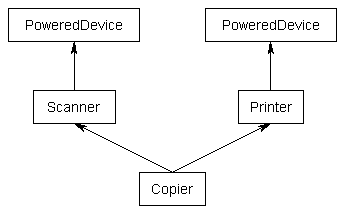
\includegraphics{rsrc/PoweredDevice2.png}
\end{center}
\item Each parent class has its own copy of the base class data members (resulting in redundant copies), and we can't call public members of the base class from the new derived class.
\item The diamond problem refers to our liking for a single instance of the base class in such cases of multiple inheritance, which is different from what happens when we try to implement such a hierarchy.
\item The solution is to use the keyword virtual while declaring the parent classes to identify them as virtual base classes:
\begin{lstlisting}[language=C++]
    class base{};
    class b1: virtual public base{};//
    class b2: virtual public base{};//without virtual in both of them, copies are made.
    class derived: public b1, public b2{};
\end{lstlisting}
\begin{itemize}
    \item Without \texttt{virtual}, each parent class maintains its copy of variables from the base class,\\
    and sizeof(derived) = (sizeof(b1)+size(b2)).
    \item With \texttt{virtual},\\ sizeof(derived) = (sizeof(b1 without b data)+sizeof(b2 without b data) + sizeof(b)+16B)
    \item The 16B are for book keeping. It can also be 8B on some systems.
    \item Note that all parent classes are prefixed with \texttt{virtual} and share ancestors, have a single copy of the ancestor's variables in the derived class.
    \item The book-keeping info grows with 8B for each new parent class. It doesn't grow with the size of the base class (or any class).
\end{itemize}
\item The construction of the base class becomes the responsibility of the derived class:
\begin{lstlisting}
class Copier: public Scanner, public Printer{
public:
Copier():PoweredDevice()/*base class*/, Scanner(), Printer(){
    //Order of constructor defintions run.
    //Base
    //base1
    //base2
    //Derived
}
}
\end{lstlisting}
\item The point above is true because of Printer, Scanner being virtual base classes. The order of constructors holds \textbf{even when single inheritance is done from a virtual base class}.

\item Accessing members of the root class, using an object of a class derived from two non-virtual sibling descendants of the root, leads to compilation errors. To avoid this, either declare the siblings as virtual descendants or use scope resolution operators (of the sibling classes, not the root!).
\end{itemize}
\section{Overloading}
TODO order of usage around operators study.
\begin{itemize}
    \item A single identifier (function name/operator) corresponds to two different implementations, based on the argument list supplied to it.
    \item Overload resolution refers to the compiler's task of selecting the most appropriate implementation when it encounters a call to an overloaded function.
    \item Note: operators can be overloaded outside classes too:
    \begin{lstlisting}[language=C++]
        //As a member function:
        Box operator+(const Box&);
        //Not as a member function:
        Box operator+(const Box&, const Box&);
    \end{lstlisting}
    \item In general, use const and \& for operands to 
    \begin{itemize}
        \item Avoid accidentally modifying them in the operation.
        \item Avoid time spent copying them around.
    \end{itemize}
    \item Most operators can be overloaded:
    \begin{center}
        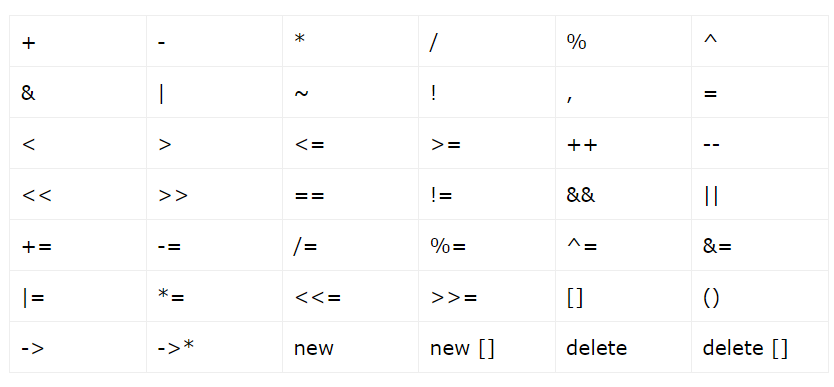
\includegraphics[width=8cm]{rsrc/overloadableops.png}
    \end{center}
    \item Operators that can't be overloaded:
    \begin{enumerate}
        \item ::
        \item .*
        \item .
        \item ?:
    \end{enumerate}
    \item Unary operators include: ++ (post,pre), -- (post,pre), -, ~ and !
\end{itemize}
\subsection{Overloading ++ (and --)}
\begin{lstlisting}[language=C++]
class Digit{
//postfix: a++ : returns an rval.
Digit operator++(int){
    ... return digit;
}
//prefix: ++a : returns an lval. (original variable)
Digit& operator++(){
    ... return *this;
}
}
\end{lstlisting}
\begin{itemize}
\item Both definitions have something unique:
\begin{enumerate}
    \item \& in the prefix definition, to ensure it returns an lvalue.
    \item (int) in the postfix definition is necessary to distinguish it from the prefix definition, as c++ doesn't support return-value-based overloading.
\end{enumerate}
\item Also note that though operator++(int) looks like ++a (prefix), it's actually for a++ (postfix).
\end{itemize}
\section{Polymorphism}
Polymorphism means a call to a member function (after resolution of overloads), can lead to different implementations being called, based on the type of object that invokes the function.
\subsection{Static Linkage}
\begin{lstlisting}[language=C++]
class Shape {
   public:
      int area() {
         cout << "Parent class area :"...
      }
};
class Rectangle: public Shape {
   public:
      int area () { 
         cout << "Rectangle class area :"...
      }
};
class Triangle: public Shape {
   public:
      int area () { 
         cout << "Triangle class area :"... 
      }
};
int main() {
   Shape *shape;
   Rectangle rec(10,7);
   Triangle  tri(10,5);
   shape = &rec;
   shape->area();
   shape = &tri;   
   shape->area();
   //both calls print "Parent class area:..."
   return 0;
}
\end{lstlisting}
Without any prefixes in the functions defined in the derived classes (that are identifiable with functions in the base class),
the compiler assumes that any calls to these functions from an object of type base*/base always needs the implementation from the parent class. This is known as static linkage or static resolution (of the function call) or early binding, as the implementation for the area function is fixed at runtime to that of the base class (for objects of or pointers to the base class).\\
Note that calls from \texttt{rec} or \texttt{tri} would have called their respective functions, not the base class' function.
\subsection{Dynamic Linkage}
Prefixing function identifiers that are shared across derived and base classes with \texttt{virtual}, allows for dynamic linkage, or dynamic resolution or late binding. With the said prefix, the compiler identifies the right implementation to call by the contents of the object or pointer being used to invoke the function. This is polymorphism.
\subsubsection{Pure Virtual Functions}
If a function is always intended to be overridden in the derived classes and there's no meaningful definition in the base class,
we can just declare the function in the base class and set it to zero to avoid compilation errors about no definition being found for
the function in the base class.
\begin{lstlisting}[language=C++]
class Shape{
    //virtual int area();
    //Above line compiles if there are no to area() from any objects of shape/derived classes.
    //In the presence of such calls, even if area() is defined in derived classes and their
    //objects are used to call area() (from the right pointer, or a pointer of type Shape*)
    //compilation errors ensue.
    //However,
    virtual int area()=0;//goes through compilation successfully.
};
\end{lstlisting}
Note:
\begin{itemize}
\item We say a function demonstrates polymorphism if we can use a pointer of the base class
to access functions of different derived classes and have different implementations
being used based on the derived class to which the object belongs. 
\item Without the virtual keyword, even if functions with identical identifiers (name
and arguments considered) are declared in derived and base classes, polymorphism is not
observed. Function calls from pointers of the base class' type call its own implementation,
not that of derived classes. 
\item Once a function is declared as virtual in a class, it demonstrates polymorphism 
across all derived descendant classes, even without the virtual keyword being present 
intermediate classes.
\item The \texttt{final} keyword can be used to throw a compilation error if a function
that we don't want any base classes to override is overridden:
\begin{lstlisting}[language=C++]
class Rectangle:public Shape{
    public:
    int area()final{
        cout<<"Rect Area"<<endl;
        return 0;
    }
};
//Now if a class called square attempts to override area, a compilation error is thrown.
\end{lstlisting}
\item Using the final keyword in a non-virtual function (that was not declared to be virtual in any of the ancestors) throws a compilation error.
\item \textbf{Object Slicing:} When an object of a derived class is assigned to an object (not a pointer) of
a base class, only members inherited from the base class are kept and the others are discarded. Thus,
all functions that may have been overridden are reverted to their definitions in the base class.
\begin{lstlisting}[language=C++]
void printarea(Shape s){
    s.area();
}
void printareaReference(Shape &s){
    s.area();//NO slicing. 
}
Shape s; Rect r;
s = r;//slicing.
Shape &s = r;
printarea(r);//slicing. prints "Shape area..."
printareaReference(r);//No slicing. prints "Rectangle area..."
\end{lstlisting}
In JAVA, and other languages where each non-primitive variable is actually a reference, object
slicing doesn't happen.
\end{itemize}
\section{Data Abstraction and Encapsulation}
The idea is to write classes with a well-defined boundary between:
\begin{enumerate}
\item Implementation: how the class works, the variables and functions it needs for its work.
\item Interface: the function calls and variables accessible to the users of the class.
\end{enumerate}
Data abstraction allows:
\begin{itemize}
\item Implementation of a class to evolve without affecting code that uses it.
\item Prohibiting users from possibly disturbing the state of the objects of the class,
which may affect correctness of its functions. Ex. A user sets the \texttt{top} pointer
inside a stack's implementation to the start of the array, without updating the length,
which is non-zero. This results in a segmentation fault.
\end{itemize}
It is enforced using access specifiers. Data encapsulation is about
bundling all the related data and functions that use it into one class,
keeping as much implementation detail from the user as possible.
\section{Abstract Classes a.k.a C++ Interfaces}
An abstract class is a class with at least one \textbf{pure virtual function}.
Such classes define an interface that all derived classes have to support (have an
implementation of).
\section{Notes from interview questions}
\begin{itemize}
    \item In multilevel inheritance (A->B->C), any function calls from an object of type C are linearly searched for up the hierarchy, and the first implementation is taken.
    \item Pointers of a parent type can hold a child, but child pointers being assigned to parent objects raises compilation errors.
    \item Pointers of a parent type can only access members (variables and functions) declared and declared public in the parent.
    \item When a derived class defines a function with the same name as some function its base class, all functions (even with different signatures) of the base class with the same name become inaccessible to objects.
    \item However, using a pointer of the base type to point to the object of the derived class, both the overridden method and the unoverridden overload of a method with the same name can be accessed.
    \item Or, using a scope resolution operator:
    \begin{lstlisting}[language=C++]
        d.Base::fun(5);//goes through.
        Base &b = d;
        b.fun(5);//goes through.
    \end{lstlisting}
\end{itemize}
\subsubsection{Initializer Lists}
\begin{itemize}
\item Initializer lists of a derived class can't
include members of the base class. They need to be initialized using the contructor of the base class.
\end{itemize}
\subsection{Destructors}
\begin{itemize}
\item The default destructor of a base class is accessible to everyone.
\item If it is overridden, it must be specified at least as protected.
\item If the destructor is declared as protected, calls to \texttt{delete baseptr}
throw compilation errors.
\item Ideally, if \texttt{baseptr}s are intended to be used for polymorphism and 
we want to avoid \texttt{delete baseptr} calls, we should set the destructor to protected.
\item Finall, if a the destructor is public, and \texttt{delete baseptr} is called, the 
destructor of any derived class object held in baseptr is not called, and the chain of destructors
starts being called from that of the baseptr's class.
\end{itemize}
\subsection{New and Delete}
TODO
\subsection{Copy Constructors}
\begin{lstlisting}[language=C++]
class Sample{
    int id;
    Sample(Sample &t)
    {
        id=t.id;
    }
};
//defines what do to do when:
Sample a,b;
a = b;//calls copy constructor of a.
\end{lstlisting}
\begin{itemize}
\item Used to intialize members of a newly created object by copying members of an already existing object.
\item It takes a reference parameter of an object of the same class.
\item This is known as copy initialization, a.k.a. member-wise initialization.
\item If not defined explicitly by the programmer, the compiler 
defines it for us.
\item The following definition of a copy constructor makes the object of this class uncopyable:
\begin{lstlisting}
class Derived{
    Derived(const Derived&) = delete;
};
\end{lstlisting}
\item Attempting to copy \texttt{Derived} objects in the code throws a compilation error.
\item Hence, \texttt{throw d} also throws a compilation error, as \texttt{throw} implies copy operations. (See Exceptions section.)
\end{itemize}
\subsubsection{Types of Copy Constructors}
\begin{enumerate}
\item Default Copy Constructor: The implementation offered by the compiler which copies the bases and members of an object in the same order that a constructor would intialize the bases and members of the object.
\item User Defined Copy Constructor: needed when an object owns pointers or non-shareable references, such as to a file. A destructor and assignment operator should also ideally be written in this case to assist in transfer/destruction of said references.
\end{enumerate}
A copy constructor is called when:
\begin{itemize}
\item An object of the class is \textbf{returned by value.}
\item An object of the class is \textbf{passed by value} as an argument.
\item An object is constructed based on another object of the same class. Ex: \texttt{Shape s1 = {1,2}; Shape s2(s1) or Shape s2 = s1;}
\item The compiler generates \textbf{a temporary object.}
\end{itemize}
Note that it's not called when a previously declared object is assigned another object. This calls the assignment operator.
\begin{lstlisting}[language=C++]
Shape s1,s2;
s1 = {1,3};
Shape s3(s1);//calls copy constructor.
Shape s4 = s1;//calls copy constructor.
s2 = s1;//calls assignment operator.
\end{lstlisting}
Note that a call to the copy constructor is not guarranteed as
the compiler performs optimizations like \textbf{return value 
optimization} and \textbf{copy elision} to avoid unnecessary 
copies where possible. (TODO)\\
Other points:
\begin{itemize}
\item Use a user-defined copy constructor when the default copy constructor results in a shallow copy (say, if some members are pointers). Deep-copy is only possible in a user-defined constructor.
\item Copy constructors can be made private, and this makes objects of the class non-copyable. It's particularly useful (as a lazy technique to avoid shallow copies) if the class has pointers of dynamically allocated resources. The right way is to write a deep-copy-constructor and make it public.
\item A copy constructor which takes the object argument by value leads to a compilation error, as at runtime it would have lead to an infinite chain of copy constructor calls.
\item Use const in the argument to make sure:
\begin{enumerate}
    \item The source object isn't accidentally modified.
    \item The copy-constructor can be called with temporary objects created by the compiler, which can't be bound to non-const references.
    \begin{lstlisting}[language=C++]
        //if copy constructor doesn't say const Shape &s1,
        Shape s2 = fun();//fun returns s2 by value.
        //the above code throws a compilation error, at the last line.
        //If const is present, it compiles.
    \end{lstlisting}
\end{enumerate} 
\item In default constructors, default constructors of parents are called before those of derived classes, but, in copy constructors, the parent's default constructors (not copy constructors are called), unless the implementation of the derived class' copy constructor specifically calls their copy constructors.
\end{itemize}
\subsubsection{Copy Elision (a.k.a. Copy Omission)} 
The compiler avoids making copies of objects (in pass by value/return by value scenarios) where possible.

\section{From LearnCPP.com}
\subsection{14.4 Const objects}
\begin{lstlisting}[language=C++]
const Date today {2020, 10, 14};//valid.
const Date today = {2020, 10, 14};//valid.
//Note that const objects must be initialized, unless a default
//constructor is defined.
\end{lstlisting}

Objects that are declared with \texttt{const} keyword (as a local variable, or a function argument) impose certain restrictions (that upon violation lead to compiler errors.):
\begin{itemize}
\item Their members variables can't be changed, neither via direct access nor calls to member functions that change them.
\item Additionally, const objects can't call non-const member functions. \texttt{const} before the definition body indicates that the member function doesn't modify the members of the class; it doesn't impose any restrictions on the returned value or aruments.
\begin{lstlisting}[language=C++]
class Date{
    //can't be called by a const object, despite not
    //altering any variables in its definition:
    void print(){
        cout<<"non-const member function.";
    }
    //can be called by const objects:
    void print2() const {
        cout<<"const member function.";
    }
}
\end{lstlisting}
\item If the declaration and definition are written separately, \texttt{const} must be present after the function signature in both places.
\begin{lstlisting}[language=C++]
class Date{
    void print() const;
};
void Date::print()const{
    ...
}
\end{lstlisting}
\item An attempt to modify the class inside a const function raises a compilation error, even inside unreachable if-blocks.
\item Within the definition of a const member function, \texttt{this} is a const pointer to a const object.
\item No constructor can be declared as a constant, as they need to modify the member variables, regardless of what their implementation says.
\item It is perfectly fine to call const member functions from non-const objects.
\item Functions can be overloaded based on whether they are const or not. So, const objects call the const variant while non-const objects call the non-const variant. This is usually done if constness changes the return value.
\begin{lstlisting}[language=C++]
//These are valid overloads:
int fun(){

};
int fun()const{

};
//These are invalid as const keyword specifiers return type.
int fun(){}
const int fun(){}
//Also note that
const int fun(){};
//is exactly the same as:
int const fun(){};
//and the two are different from
int fun()const{};
\end{lstlisting}
\end{itemize}
\subsection{14.6 Access functions}
\begin{itemize}
\item Trivial member functions to access selectd private data members.
\item Of two types: Setters (mutators) and getters (accessors).
\item Getters are made const so they can be called on const objects while setters have to be non-const.
\item For efficiency, getters can be written to return constant lvalue references, instead of returning by value:
\begin{lstlisting}
const std::string &getName()const{return m_name;}
\end{lstlisting}
\item Note that such functions' returned references become invalid the moment the object is destroyed. So, the references should not be stored (and accessed) beyond the lifetime of the object.
\begin{lstlisting}
const std::string & ref = createEmployee().getName();
//we store the reference to a property in the rvalue implicit
//temporary object, created by the compiler.
//accessing ref later leads to undefined behaviour. 
\end{lstlisting}
\item References returned from functions to private members should be constant; otherwise, they permit direct modification of private members.
\end{itemize}
\subsubsection{Ref-qualifier overloads}
\begin{lstlisting}
const std::string& getName() const & { return m_name; } // when called on an lvalue (single &), return member by reference
const std::string getName() const && { return m_name; } // when called on an rvalue (double &&), return member by value
// Alternately, we can disable the use of a member functions for rvalue objects
const std::string& getName2() const && = delete;         // when called on an rvalue, emit a compilation error
\end{lstlisting}
\section{Friends}
A friend is a class or function (member or non-member) that has been granted full access to the private and protected members of another class. Using friends, classes can selectively give full access to their members without unnecessary impacts.\\
The friendship is established by (declared in) the class removing its access control for some other entity.
\subsection{Friend (non-member) Functions}
With non-member functions, an object of the class must be accepted as an argument to access the relevant data.
\begin{lstlisting}
class Shape{
    int area;
    friend double paintcost(const Shape& shape);
};
double paintcost(const Shape& shape){
    return shape.area*costunit;//accesses private member and compiles.
}
\end{lstlisting}
\begin{itemize}
\item Note that the friend function can also be defined inside the class, and remain a non-member function because of the \texttt{friend} keyword.
\item A function can be a friend of multiple classes, all of 
which appear in its argument list. These are used when it makes 
less syntactic sense to make the function a member of either 
class.
\begin{lstlisting}
friend void printWeather(const Temperature& temp, const Humidity& hum){
    //access private members of both temp and hum at once.
}
\end{lstlisting}
\item Access specifiers make no difference to the availability of friend functions as they are non-members anyways.
\item Friend functions should also use the class' interface where possible, instead of directly accessing data, as this insulates them from future change in the class.
\end{itemize}
\subsection{Friend Classes and Member Functions}
\begin{itemize}
    \item Friend classes can access private and protected members of another class.
\begin{lstlisting}
class Storage{
    //private members here.
    friend class Display;
    //Display declared as a friend of storage.
    //Display accesses all members of storage.
    //Note: no forward declaration required.
};
class Display{
    void print(const Storage& storage);
}
\end{lstlisting}
\item Friendship is not reciprocal.
\item Friendship is not transitive.
\item Frienship is not inherited. Classes derived from a friend are not friends.
\end{itemize}
\subsubsection{Friend Member Functions}
\begin{itemize}
\item One point worth prattling about is that the compiler needs to have seen the declaration of a member function before it can be declared as a friend somewhere using the syntax below:
\begin{lstlisting}
class Storage{
    //private members.
    friend void Display::displayStorage(Storage &storage);
    //compiler should have seen displayStorage in Display 
    //before this line.
};
\end{lstlisting} 
\item This implies the compiler should have encounted the \textbf{full definition of the class} to which the member function belongs, not just a forward declaration.
\item Additionally, to use members of the class where friendship is declared (\texttt{Storage}), it should have been declared before the definition of the friend member function.
\item A better solution is of course to split the code up into separate files.
\end{itemize}
\chapter{C Stuff}
\section{Calloc vs Malloc}
\begin{center}
\begin{tabular}{| p{8cm} | p{8cm} |}
    \trow{Malloc}{Calloc}
    \trow{\texttt{(void*) malloc(NumBytes)}}{\texttt{(void*) calloc(NumElems, ElemSizeInBytes)}}
    \trow{Stands for memory allocation.}{Stands for clear memory allocation.}
    \trow{Returned memory block has garbage values.}{Returned memory block is initialized to 0.}
    \trow{Faster than calloc.}{Slower than malloc.}
    \trow{Doesn't involve memory overheads.}{Involves some memory overheads.}
    \hline
\end{tabular}
\end{center}
\chapter{More C++ Stuff}
\section{Templates from LearnCpp.com}
\begin{itemize}
\item Templates are declarations of functions of classes with placeholder types.
\item Placeholder types aka, type template parameters, aka template types.
\item A placeholder type is not known at the definition of the template, but is decided at a call to the template.
\item Once a template is written, the compiler can use it to generate as many overloaded entities as needed, using concrete types.
\item C++ allows three kinds of template parameters:
\begin{enumerate}
    \item Type template parameter: represents a type.
    \begin{itemize}
        \item Use keywords \texttt{typename} or \texttt{class}.
        \item \texttt{typename} can be replaced by any type, primitive or a class.
        \item TODO: are the two equivalent?
    \end{itemize}
    \item Non-type template paramater: represents a constexpr value.
    \item Template template paramater: represents a template.
\end{enumerate}
\item Templates are analogous to stencils.
\item Templates can work with types that didn't even exist when they were written.
\item It's common convention to use uppercase letters for template parameters.
\end{itemize}
\subsection{Function Templates}
\begin{itemize}
\item Example:
\begin{lstlisting}
template<typename T>
T max(T x, T y){
    return (x<y)?y:x;
}
// signature is now: T max<T>(T x, T y);
\end{lstlisting}
\item A function call looks like: \texttt{max<int>(a,b);}
\item It is necessary to specify T in every call to \texttt{max<T>}.
\item When the compiler encounters a call to \texttt{max<int>}, and it doesn't have a corresponding definition yet,
it uses the template to create a function for the type selected.
\item This is known as \textbf{(Function) (Template) Instantiation}.
\item \textbf{Implicit instantiation} refers to instantiation due to a function call statement.
\item Instantiated functions are called a \textbf{function instance} or \textbf{template function}.
\item Function instances are normal functions in all regards.
\item Function instantiation is a compiler task, and thus happens during compilation.
\end{itemize}
\subsubsection{Template Argument Deduction}
\begin{itemize}
\item If all the template type parameters appear in the function's argument, and 
the arguments we pass to the function have the right type (without the need for coercion),
then we can omit the type specification in the function call statement:
\begin{lstlisting}
max<int>(a,b);
max<>(a,b);//Compiler only studies templates for finding an overload.
max(a,b);//compiler first studies non-template declarations of max, followed by templates. 
\end{lstlisting}
\item The order of checking for overloads before templates allows for type-specific optimizations in generic functions.
\item So, if the type parameters are deducible from the arguments and we want to use the type-specific, non-template
overload of the function, use \texttt{max(a,b)}, but use \texttt{max<>(a,b)} if you want to use the template overload
for some reason.
\item For instantiated functions to successfully compile, it is necessary for their bodies to not invoke any functions or operators not defined for the types being inferred from the function calls.
\item Note that the compiler generates instantiated functions so long as they make sense syntactically. It is our responsibility to ensure semantic sanity is maintained.
\item We can disallow particular template overloads using \textbf{function template specialization} like so:
\begin{lstlisting}
template <typename T>
T addOne(T x)
{
    return x + 1;
}

// Use function template specialization to tell the compiler that addOne(const char*) should emit a compilation error
template <>//empty type parameter list, NOT <char*>
const char* addOne(const char* x) = delete;
\end{lstlisting}
\item Attempt to use deleted function instances raises compilation faults.
\item It is common practice to put the entire template declaration and definition in header files, rather than just the declaration, as all cpp files need to know the template exists for their function calls to instantiate the relevant overloads from the template.
\item Functions implicitly instantiated from templates are implicitly inline; inline functions can be defined in multiple files, so long as their definitions are identical.
\item TODO: inline functions.
\item The template themselves are not inline, which is a concept that only applies to functions and variables.
\item Generic programming refers to the practice of using templates and associated template parameters (generic types).
\item There are some drawbacks to template programming:
\begin{itemize}
    \item Code bloat and slow compile times: As the compiler instantiates a function for each call with a unique set of arguments, even compactly written templates cause the two problems.
    \item Error messages from using templates are much more convoluted than regular error messages.
\end{itemize}
\end{itemize}
\subsubsection{Multiple Template Types}
\begin{itemize}
\item Note that a function call with different types being passed in place of T without explicitly mentioning \texttt{<T>} raises compilation errors.
\begin{lstlisting}
template <typename T>
T max(T x, T y)
{
    return (x < y) ? y : x;
}
int main()
{
    std::cout << max(2, 3.5) << '\n';  // compile error
}
\end{lstlisting}
\item The compiler doesn't know which overload to refer to and which argument to coerce.
\item Type coercion is done only in function overloads, \textbf{not in template argument deduction}.
\item Note about function overloading:
\begin{itemize}
\item This compiles but isn't sound:
\begin{lstlisting}
int mymax(int x,int y)...
mymax(2,2.5);//returns 2
mymax(2.1,2.5);//returns 2
\end{lstlisting}
\item This compiles and is sound:
\begin{lstlisting}
double mymax(double x,double y)...
mymax(2,1);//returns 2. Note that double arguments are trivially sound.
mymax(2,2.5);//returns 2.5.
\end{lstlisting}
\item This doesn't compile:
\begin{lstlisting}
int mymax(int x,int y)...
double mymax(double x,double y)...
mymax(2,2.5);//compiler error, ambiguous overload.
\end{lstlisting}
\end{itemize}
\item There are three ways to allow this mixing of types in templates.
\begin{enumerate}
\item Static Casting the arguments in a function call, without specifying the template type.
\begin{itemize}
\item Must use static cast \texttt{static\_cast<T>(var)} instead of dynamic casting \texttt{(type T)(var)}, which happens at runtime, because we need the type to be casted at compile time, to find the right template.
\end{itemize}
\item Just provide the template type and avoid the need for template argument deduction.
\item Declare function template types with multiple type parameters. (Discussed below.)
\end{enumerate}
\item Allow multiple types in the argument list and use auto to ensure arithmetic conversions don't lose data.
\begin{lstlisting}
template <typename T, typename U>
auto max(T x, U y)
{
    return (x < y) ? y : x;
}
//now this works for (T,T) and (T,U) instances.    
//C++ 20 introduces abbreviated function templates:
//Below is a shorthand for the above beast:
auto max(auto x, auto y)
{
    return (x < y) ? y : x;
}
//should be used only if x and y are allowed to be of different types.
\end{lstlisting}
\end{itemize}
\subsection{Non-type Template Parameters}
\begin{itemize}
\item Serve as placeholders for constexpr values passed in during a function call.
\item A non-type template parameter can have be one of:
\begin{enumerate}
    \item An integral type
    \item An enumeration type
    \item \texttt{std::nullptr\_t}
    \item A floating point type (C++ 20)
    \item A pointer or reference to:
    \begin{itemize}
        \item An object
        \item A function or member function.
        \item A literal class type (C++ 20).
    \end{itemize}
\end{enumerate}
\item Example of usage:
\begin{lstlisting}
bitset<8> b;
\end{lstlisting}
\item Syntax:
\begin{lstlisting}
template <int N> // declare a non-type template parameter of type int named N
void print()
{
    std::cout << N << '\n'; // use value of N here
}
\end{lstlisting}
\item On seeing a call to \texttt{print<5>()}, the compiler instantiates a print function with N=5.
\item One application is in creating data structures whose size is fixed at compile time.
\item One other application is in static asserts for values passed as non-type template parameters. For example, in a sqrt function.
\item Type conversion of non-int parameters is often performed:
\begin{lstlisting}
print<'c'>();//compiles with casting 'c' to int.
\end{lstlisting}
\item Though only some types of constexpr conversions are allowed:
\begin{itemize}
    \item Integral promotions (ex. char to int).
    \item Integral conversions (char to long or int to char).
    \item User-defined conversions (some custom class to int).
    \item Lval to Rval conversions.
\end{itemize}
\end{itemize}
\section{Exceptions from LearnCpp.com}
\begin{itemize}
\item The primary issue with error-handling without exceptions is that
the error-handling code ends up intricately linked to the normal control
flow of code; constraining both how the code is laid out and how errors can 
be reasonably handled.
\item Exceptions allow decoupling of error-handling code from the regular flow of control.
\item Three C++ keywords are used for this:
\begin{enumerate}
\item \texttt{throw} It is followed by an object of any kind (int/double/class).
\item \texttt{try} Encloses the block of code that can raise an error.
\item \texttt{catch} Specifies the object to be expected if an error is thrown and what to do with it.
\end{enumerate}
\item Each try block can have many catch blocks, each expecting a different 
type of object to be thrown, but must have at least one.
\item Execution resumes normally at the end of the catch block.
\item Exceptions of non-primitive types should be caught in const references to avoid unnecessary copies.
\item The variable name of a parameter can be excluded if it is not used inside the catch block.
Though it's type must be specified nonetheless.
\item The compiler searches for matching enclosing "catch" blocks for a thrown exception up the program,
until it is caught. If no catch block is found, the program fails with an exception error.
\item The compiler only ever casts derived classes of exceptions to their parents classes, but it never
casts between primitive types.
\item The catch block can serve one of four purposes:
\begin{enumerate}
\item Convey the caught error to the user in a neat way, say, by printing to the console.
\item Return a value or error code back to the current function's caller.
\item Throw another exception, to be caught by an outer try-catch block.
\item Terminate the program cleanly.
\end{enumerate}
\end{itemize}
\subsection{Stack unwinding}
\begin{itemize}
\item If the current function doesn't have a try-catch block enclosing the thrown exception,
the current searches down the call stack to find the first enclosing try-catch block.
\item On finding said block, the stack unwinds (locals are popped off) until the control can 
resume in the stack's state of the function that contains said catch block.
\item If no catch block is found all the way to main, the program terminates \textbf{without} unwounding the stack.
\item This may lead to trouble if some locals have non-trivial destructors.
\item The stack not being unwound allows retention of all the debug info related to the exception.
\item Behold the catch-all handler, that catches all exceptions:
\begin{lstlisting}
    try{
        //exception throwing code.
    }
    catch(int a){

    }
    catch(...){
        cout<<"All non-int exceptions lead here"<<endl;
    }
\end{lstlisting}
\item The catch-all handler should be the last block in the catch block chain,
to allow for specific error-handling as much as possible.
\end{itemize}
\subsection{Exceptions within classes}
\begin{itemize}
\item If a constructor of class A throws an exception, all the initialized members call their 
respective destructors, but ~A() is never called, as construction never succeeded.
\item This can lead to missed cleanup for resources that had been allocatd in A() before the exception.
\item However, if each resource that demands cleanup was declared inside a member of A, that had
its own destructor with the requisite cleanup code, the cleanup would go through.
\item However, creating a class to manage each resource, and be a member in A, isn't efficient.
\item STL provides classes that have destructors for cleanup:
\begin{itemize}
    \item \texttt{std::unqiue\_pointer<T>} : for pointers that are freed on destruction.
\end{itemize}
\end{itemize}
\subsection{Classes for Exceptions}
\begin{itemize}
\item Seeing as primitive types convey vague information about the error, it is
preferable to define classes that are meant to be thrown around.
\item A hierarchy of such classes is useful and often done.
\item Catch blocks with an argument of a base class also catch all errors of derived classes
without slicing, if the argument is a reference argument, and with slicing otherwise.
\item If the base catch block precedes the derived catch block, the base catch block executes.
\item Otherwise, the derived catch block executes.
\item Hence, catch blocks for derived classes should be written before (above) those for base classes.
\item All of the exceptions thrown by STL in C++ are of classes derived from \texttt{std::exception}.
\begin{lstlisting}
catch(std::exception &e){
    cout<<e.what()<<endl;//prints the error description.
}
\end{lstlisting}
\item Note that \texttt{e.what()} messages vary across compilers.
\item A common derived class to use is \texttt{std::runtime\_error("message for what")}.
\item We can of course further extend the STL class hierarchy in our codebase.
\item Rethrowing exceptions is a common practice.
\item If an exception is caught by an argument that is of a class less-derived than the exception,
the right way to rethrow the exception is \texttt{throw;} (an empty throw statement).
\item A statement like \texttt{throw baseException;} slices the derived exception class.
\end{itemize}
\subsection{Storing Exceptions}
\begin{itemize}
\item When an exception is thrown, its data is initially on the local stack.
\item If the stack needs to be unwound for it to be caught, the compiler copies
its data to memory location reserved for exceptions off the stack, until
a catch block is encountered.
\end{itemize}
\subsection{Function Try Blocks}
\begin{itemize}
\item One use case of function try blocks is when we want to catch
an exception thrown by the constructor of a base class, in the constructor of the 
derived class.
\begin{lstlisting}
class B : public A
{
public:
    B(int x) try : A{x} // note addition of try keyword here
    {
        //usual constructor stuff
    }
    catch (...) // note this is at same level of indentation as the function itself
    {
            // Exceptions from member initializer list or constructor body are caught here
            std::cerr << "Exception caught\n";
            throw; // rethrow the existing exception
    }
};
\end{lstlisting}
\item Note that function level catch blocks \textbf{for constructors} must throw an exception.
They are not allowed to resolve and just consume exceptions.
\item Implicit rethrows are called at the end of the catch-block, hence it is better to generally avoid
letting control get to the end of these catch blocks.
\begin{center}
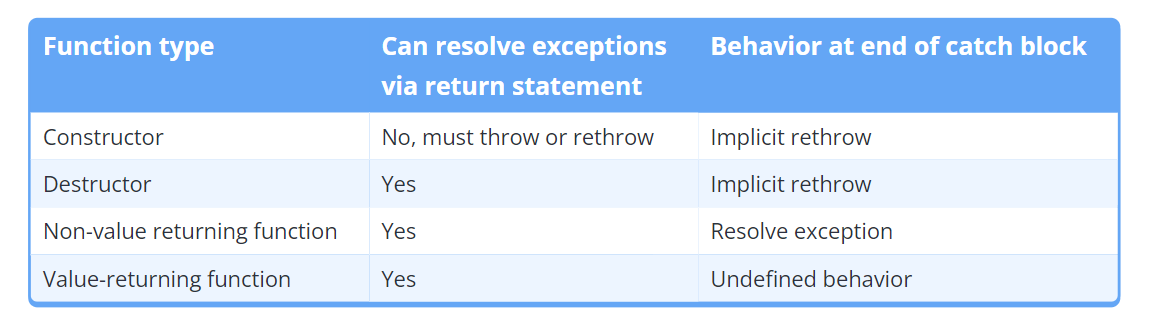
\includegraphics[width=13cm]{rsrc/functiontrycatch.png}
\end{center}
\item We shouldn't use the catch block to clean up resources of a failed constructor, as the object was never created if an exception was thrown.
\end{itemize}
\subsection{Common Design Mistakes}
\begin{itemize}
\item Cleanup calls to resources established and used inside a try block should be outside the catch block, so they're called in normal execution, and in exceptional execution. This is assuming that control exits the catch block.
\begin{lstlisting}
try
{
    openFile(filename);
    writeFile(filename, data);
}
catch (const FileException& exception)
{
    std::cerr << "Failed to write to file: " << exception.what() << '\n';
}
// Make sure file is closed
closeFile(filename);
\end{lstlisting}
\item Additionally, the variables must be in scope for the cleanup calls, and must be declared outside the try block.
\item Or as discussed earlier, we can uses STL classes like \texttt{unique\_pointer<T>} or other resource
classes with destructors that perform the cleanup.
\item Generally abstain from using exceptions in destructors as an exception thrown during stack unwounding
"confuses" the compiler between continuing the unwound or handling the exception.
Instead, write the error to a log file.
\item It should be noted that exceptions come with performance costs such as:
\begin{enumerate}
    \item Mainly: the expensive operation of unwinding the stack on an exception and finding the suitable catch block.
    \item An heavier executable.
    \item The program runs slower due to additional checks.
\end{enumerate}
\item Some compilers implement \textbf{zero-cost exceptions}, where the runtime cost
 of exception-handling is zero for a no-exception scenario, but incurs large penalties
 in exceptional scenarios.
\end{itemize}
\subsection{Exception Specifications}
\begin{itemize}
\item Language mechanism to document what kind of exceptions a function can throw, in its declaration.
\item The \texttt{noexcept} keyword in a function declaration guarrantees that the function won't throw an exception.
\begin{lstlisting}
void doSomething() noexcept{
    //body that can't throw any exception out.   
}
\end{lstlisting}
\item If a \texttt{noexcept} function is overridden,
the overriding function should also be declared as \texttt{noexcept}.
\item If at runtime, an exception is emitted from a \texttt{noexcept} function,
\texttt{std::terminate()} is called immediately, even if there exist handlers around
the function call.
\item The promise of \texttt{noexcept} is contractual; it is not enforced by the compiler.
\item Functions differing only in there exception values (like those differing only in their 
return values) can not be overloads of each other; they are all the same.
\item The noexcept operator can be used to store variables conveying whether a function or
expression can potentially throw errors or not:
\begin{lstlisting}
void foo() {throw -1;}
void boo() {};
void goo() noexcept {};
struct S{};
constexpr bool b1{ noexcept(5 + 3) }; // true; ints are non-throwing
constexpr bool b2{ noexcept(foo()) }; // false; foo() throws an exception
constexpr bool b3{ noexcept(boo()) }; // false; boo() is implicitly noexcept(false)
constexpr bool b4{ noexcept(goo()) }; // true; goo() is explicitly noexcept(true)
constexpr bool b5{ noexcept(S{}) };   // true; a struct's default constructor is noexcept by default
\end{lstlisting}
\end{itemize}

\chapter{DSA Revision Notes}
\section{Stacks, Queues, Linked Lists}
\begin{itemize}
\item Implementation of stack, queue, deque usually involve maintaining a
fixed-size array and a pointer to the top/front/back of the queue that moves around.
\item The growth strategies for a stack's underlying array are:
\begin{itemize}
    \item Growth: f(N) = 2N;
    \item Tight: f(N) = N+c;
\end{itemize}
\item Push operation that call growing the underlying array cost f(N)+N+1 units.
\item 
\end{itemize}
\section{Hash Tables}
\begin{itemize}
\item Load factor $\alpha = n/m$, where the hash table has $m$ slots (unique indices)
and holds $n$ elements. $\alpha = $ average number of elements in each slot.
\item A hash function maps the keys of a hash table to its indices.
\item Hash functions are the composition of:
\begin{enumerate}
    \item Hash codemap: $KeySet \Longrightarrow Z$
    \item Compression map: $Z \Longrightarrow [0,1,...N-1]$
\end{enumerate}
\item Both have to deterministic and dependent on the key.
\item Strings are usually hashed using polynomials, with the characters
as coefficients. Common points of evaluation of polynomials are
x = 33, 37, 39 or 41.
\item Some common compression maps:
\
begin{itemize}
    \item $h(z) = z \% m$, where m is prime (~not too close to powers of 2.) m=$b^e$ makes for a bad compression map.
    $x \% 2^e$ gives last e bits of x.
    \item $h(z) = floor(m(fractional(zA)))$, where A $\in$ (0,1) and m = size of the table.
    \item Often use m = $2^p$ for above.
    \item Fibonacci hashing involves using A = $\frac{\sqrt{5}-1}{2}$
    \item $h(z) = |ak+b| mod m$ where a,N are coprime.
\end{itemize}
\subsection{Universal Hashing}
\begin{itemize}
\item A solution to the idea of adversarial choices of elements for a determined hash function.
\item A collection H of hash functions is universal if \\
For a randomly chosen h $\in$ H and two keys $k$ and $l$,\\
$P(h(k)=h(l)) < 1/m$
\end{itemize}
\subsection{Collision Resolution}
\subsubsection{Chaining}
\begin{itemize}
\item Each key is mapped to a linked list with elements that share the key.
\item Chaining is the most time efficient collision resolution method.
\item Linked lists can be sorted if necessary.
\item Search time = O($\alpha$).
\end{itemize}
\subsubsection{Open Addressing}
\begin{itemize}
\item Allows storage of at most m elements.
\item Introduce NULL elements. Use an array of size m, initialized to NULLs.
\item Systematically probe slots when searching for an element.
\item Modify the hash function to take the probe number i as the second parameter.\\
$h:\Longrightarrow Keyset \times {0, 1, 2 ... m-1}$
\item Hash function determines the sequence of slots to be examined for a given key.
\item ${h(k,0), h(k,1)...h(k,m-1)}$ is a permutation of ${0,1, ... m-1}$
\item Variations of probing include:
\begin{enumerate}
    \item Linear probing
    \begin{itemize}
        \item if h(k) is used, find next empty slot for insertion.
        \item Use a tombstone marker to delete elements, so later search queries can read the tombstone and check further elements.
        \item For deletion, search all next slots where h(slot value) = h(k) or slot value == tombstone.
        \item Rehash if there are too many tombstones.
        \item Inserts are allowed to use tombstones.
    \end{itemize}
    \item Double hashing
    \begin{itemize}
        \item set h1(k) = initprobe and h2(k) = offset.
        \item Search for empty slots starting at initprobe, in offsets of h2(k) mod m.
        \item Avoid functions h2(k) which can be give zero.
        \item If m is prime, this method examines every slot in the table.
        \item Expected number of probes to find an empty slot = $\frac{1}{1-\alpha}$ (Or an unsuccessful search.)
    \end{itemize}
\end{enumerate}
\end{itemize}
\section{Trees}
\begin{itemize}
\item In a tree, degree of a node may refer to the number of children it has.
\item \textbf{Binary Tree}: An ordered tree with each node having at most two children.
\item \textbf{Complete Binary Tree}: Each level i has $2^i$ nodes, i = 0, 1, ... h.
\begin{itemize}
    \item \# Leaves = $l$ = $2^h$; Total nodes = n = $2^{h+1} - 1$; \# Internal nodes = m = $2^{h}-1 = l - 1$
    \item height = h = $log_2(l) = log_2((n+1)/2)$
\end{itemize}
\item If a binary tree has n nodes,
\begin{equation*}
n \le 2^{h+1} - 1 \implies n-1 \le h \le log_2((n+1)/2)
\end{equation*}
\begin{equation*}
1 \le l \le m+1, l = n-m \implies l \le \frac{(n+1)}{2}
\end{equation*}
\end{itemize}
\subsection{Binary Search Tree}
\begin{itemize}
\item Structure used for ordered dictionaries, where the keys are stored
in a binary tree.
\begin{lstlisting}
Tree search(Tree t,Value v){
    if(t->value==v){
        return t;
    }
    else if(t->value < v){
        if(t->left){
            return search(t->left,v);
        }
        return NULL;
    }
    else{
        //t->value > v
        if(t->right){
            return search(t->right,v);
        }
        return NULL;
    }
}
\end{lstlisting}
\item Inorder traversal of a BST gives a sorted projection of all the keys. This is called BST-sort.
\item Has the same complexity cases as quick-sort:
\begin{itemize}
    \item WCS: O($n^2$)
    \item BCS: O($nlogn$)
    \item Average over $n!$ permutations: O($nlogn$)
\end{itemize}
\item Method implementations:
\begin{enumerate}
\item Replace: Given x,y and parent(x), replace x by y as a child of parent(x).
\begin{lstlisting}
void replace(Node*x, Node*y, Node*px){
    if(px->left==x){
        px->left = y;
    }
    else{
        //(px->right==x)
        px->right = y;
    }
}
\end{lstlisting}
\item Search: as given above.
\item Insert: search for node in tree, insert as a child where NULL is found.
\item Successor:
\begin{lstlisting}
Node *n successor(Node *x, Node *n){
    if(x->right){
        return leftMostChild(x->right);
    }
    else{
        Node *y = parent(x,n);
        while(y!=NULL && x==y->right){
            x = y;
            y = parent(x,n);
        }
        //y == root or y is closest ancestor such that x is in y->right.
        return y;
    }
}
\end{lstlisting}
\item Deletion:
\begin{lstlisting}
void delete(Node *x, Node *n){
    if(!(x->left&&x->right)){
        //x has at most one child.
        Node *y = parent(x,n);
        if(y->left==x){
            y->left = oneChildOf(x);//may return null if x has no children.
        }
        else if(y->right==x){
            y->right = oneChildOf(x);
        }
    }
    else{
        //x has two children.
        Node *s = Successor(x,n);
        delete(s,n);
        Node *y = parent(x,n);
        //transfer the children
        s->right = x->right;s->left = x->left;
        if(y->left==x){
            y->left = s;
        }
        else if(y->right==x){
            y->right = s;
        }
    }
}
\end{lstlisting}
\end{enumerate}
\end{itemize}
\subsection{Traversals}
\begin{enumerate}
\item Pre-order: Do me pre my children; process each node before its children are processed.
\begin{lstlisting}
void preorder(Node n){
    process(n);
    for(Node &u:n.children){
        preorder(u);
    }
}
\end{lstlisting}
\begin{itemize}
    \item Used in reading documents, webpages.
\end{itemize}
\item Post-order: Do me post my children; process each node after its children are processed.
\begin{lstlisting}
void postorder(Node n){
    for(Node &u:n.children){
        postorder(u);
    }
    process(n);
}
\end{lstlisting}
\begin{itemize}
\item Used by the disk-usage command and evaluation of arithmetic expressions.
\end{itemize}
\item In-order: Do me between my children; process left children first,
followed by the given node, followed by the right children.
\begin{lstlisting}
void inorder(Node n){
    for(Node &u:n.leftchildren){
        inorder(u);
    }
    process(n);
    for(Node &u:n.leftchildren){
        inorder(u);
    }
}
\end{lstlisting}
\item Eulerian: Generic traversal combining pre-, post- and in-order traversals.
\begin{lstlisting}
void eulerian(Node n){
    process(n);//First process
    for(Node &u:n.leftchildren){
        eulerian(u);
    }
    process(n);//Second process
    for(Node &u:n.leftchildren){
        eulerian(u);
    }
    process(n);//Third process.
}
\end{lstlisting}
\end{enumerate}
\subsection{AVL Trees}
\begin{itemize}
\item They are aka height-balanced binary search trees.
\item If $h(n)$ denotes the height of the tree rooted at n:
\begin{center}
    $h(n) = 1+max(h(n\rightarrow left),h(n\rightarrow right))$\\
    $h(n) = 1 \implies $ n is a leaf.\\
\end{center}
\item Define the balance factor of a node as:
\begin{center}
    $BF(n) = h(n\rightarrow right) - h(n\rightarrow left)$
\end{center}
\item $\forall n \in \{Internal Nodes\}, |h(n\rightarrow right)-h(n\rightarrow left)| \le 1$
\item $h(root) \le log_{\phi}(n)$
\item If the leaf closest to the root is at level k:
\begin{enumerate}
    \item $h(root) \le 2k-1$
    \item All nodes at levels 1...k-2 have 2 children.
    \item 2 $\implies$ n $ \ge 2^k - 1 $
    \item 1, 3 $\implies 2^{k-1} \le n \le 2^{2k-1}$
    \item 4 $\implies 2^{(h-1)/2} \le n \le 2^{h}$
\end{enumerate}
\item In an AVL tree of height h,
\begin{enumerate}
    \item The leaf closest to the root is at level $\ge (h+1)/2$.
    \item On the first $(h-1)/2$ levels, AVL tree is complete (full).
    \item $ 2^{(h-1)/2}\le n \le 2^{h}$
\end{enumerate}
\item Method implementations:
\begin{enumerate}
\item Update: (private) method to update height values and balance factor values across the tree (or subtree passed as argument.)
\item Rotaion: operation used in insertion and deletion for balance restoration.
\begin{center}
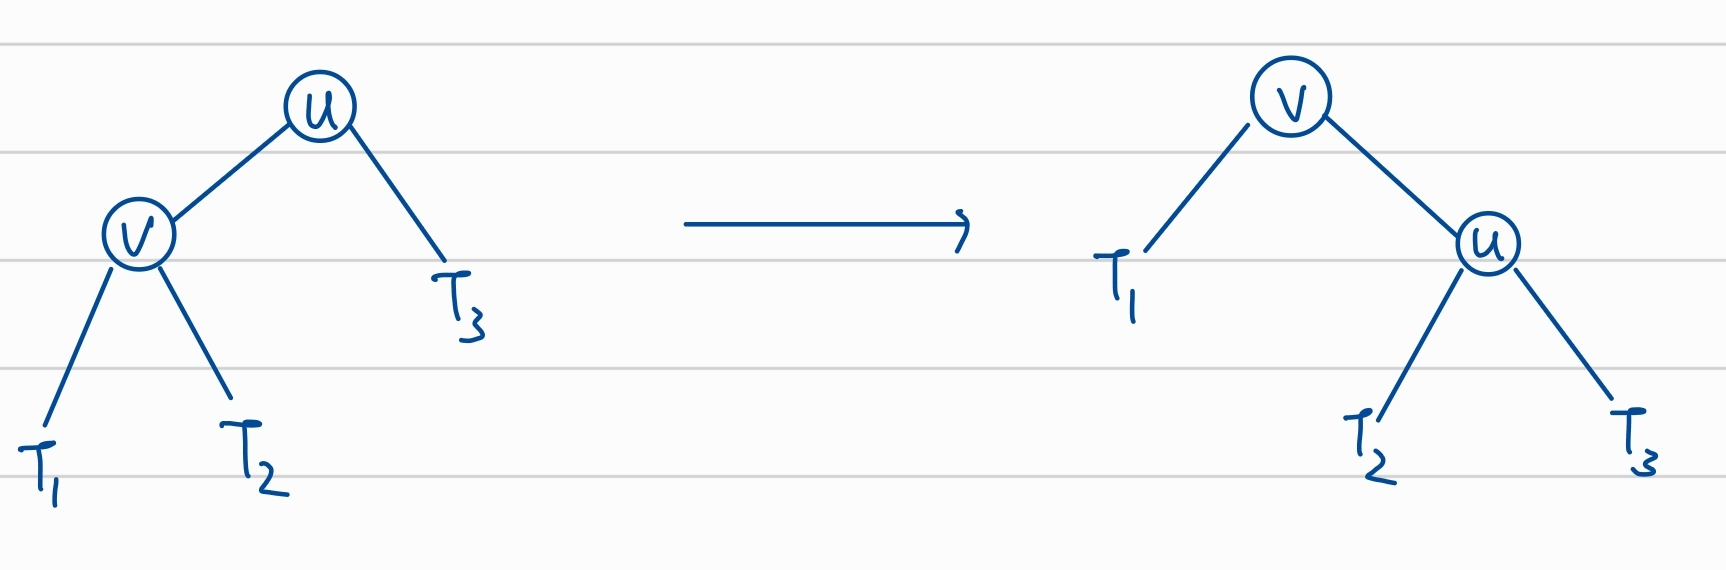
\includegraphics[width=8cm]{rsrc/AVL-rotation.jpg}
\end{center}
\begin{itemize}
\item Either structure being a valid BST implies the other is a valid BST.
\end{itemize}
\begin{lstlisting}
void rotate(Node* u,Node* v){
    //u is the parent to v.
    Node *p = parent(u);
    if(u->left==v){
        u->left = v->right;
        v->right = u;
        if(p->left==u){
            p->left = v;
        }
        else{
            p->right = v;
        }
    }
    else{
        u->right = v->left;
        v->left = u;
        if(p->left==u){
            p->left = v;
        }
        else{
            p->right = v;
        }
    }
}
\end{lstlisting}
\item Insertion: O(logn)
\begin{lstlisting}
void insert(Node *n, Value x){
    PathTraversed path = bstInsert(n,x);
    //path.last = x's node.
    //find closest ancestor of x that is imbalanced.
    //imbalance is possible because of a height increment.
    Node *top, *mid, *bot;
    bot = path.back();//x's node.
    mid = parent(bot);
    top = parent(mid);
    //top will point to the imbalanced node.
    //top->mid->bot belongs to the path.
    while(balanced(top) && parent(top)!=top){
        //root check condition.
        path.pop_back();
        back = mid;    
        mid = top;
        top = parent(top);
    }
    if(!balanced(top)){
        if(BF(top)*BF(mid)>=0){
            //left-left or right-right cases.
            rotate(top,mid);
            //balanced.
        }
        else if(BF(top)*BF(mid)<0){
            //left-right or right-left cases
            rotate(mid,bot);
            rotate(top,bot);
            //balanced.
        }
    }
}
\end{lstlisting}
\item Deletion: O(logn) We follow a similar strategy to deletion in BSTs, followed by recursive balancing.
\begin{lstlisting}
void delete(Node*n, Node* x){
    Node *z = parent(x,n);
    //if its the root, the pointer is modified.
    if(!(x->left && x->right)){
        replace(x,oneChildOf(x),z);
    }
    else{
        //x has two children.
        Node *s = successor(n,x);
        delete(n,s);
        replace(x,s,parent(x));
        z = parent(s,n);
    }
    while(parent(z)!=z){
        while(balanced(z) && parent(z)!=z){
            //find first imbalanced ancestor until root.
            z = parent(z);
        }
        y = childWithLargerHeight(z);
        x = childWithLargerHeight(y);
        if(BF(z)*BF(y)>=0){
            rotate(z,y);
        }
        else{
            rotate(y,x);
            rotate(z,x);
        }
    }
}
\end{lstlisting} 
\begin{itemize}
\item Insertion is quicker because there's only one point where rebalancing is necessary, whereas in deletion, the imbalance may be transferred higher up the tree.
\end{itemize}
\end{enumerate}
\end{itemize}
\section{String Stuff}
The common problem of finding a pattern P in a text T (|T| > |P|)
can be solved efficiently by:
\begin{enumerate}
    \item Either preprocessing the pattern (KMP)
    \item Or preprocessing the text (Tries)
\end{enumerate}
The latter is preferred if multiple patterns are searched for a in a single piece of text.
\subsection{KMP}
\begin{lstlisting}
vector<int> kmp(string t, string p){
    int l = p.size();
    int n = t.size();
    //this lps implementation is inefficient. O(l^3).
    vector<int> lps(l,0);//lps[0,1,...l-1].
    //lps[0] = 0.
    for(int i=2;i<=l;i++){
        for(int j=1;j<i;j++){
            if(p.substr(0,j)==p.substr(i-j,j) && (i==l || (p[j]!=p[i]))){
                lps[i-1] = max(lps[i-1],j);
            }
        }
    }
    int j = 0, i=0;
    vector<int> matches = {};
    for(;i<l && j<n;){
        if(t[j]!=p[i]){
            //mismatch
            if(i==0){
                j+=1;
            }
            else{
                i = lps[i-1];
            }
        }
        else{
            //match=>increment both.
            i++;
            j++;
            if(i==l){
                i = lps[i-1];
                matches.push_back(j-l);
            }
        }
    }
    return matches;
}
\end{lstlisting}
\subsubsection{Linear Time LPS}
It's complicated man. Maybe do this later.
\section{Tries}
\begin{itemize}
\item Tries are meant to store data indexed by strings from a fixed set of characters.
\item Said data can be the occurrences of the index string in a large body of text.
\item A generic implementation is give below:
\begin{lstlisting}
class Trie{
    int charindex(char c);//each char mapped to an integer,
    vector<Trie*> chars = vector<Trie*>(numChars,NULL);//integers indexing a Trie pointer,
    Data data;//initialized to empty.
    void insert(string index,Data data){
        int i = 0;
        Trie* t = this;
        while(i<index.size()){
            if(!t->chars[charindex(index[i])]){
                t->chars[charindex(index[i])] = new Trie;
            }
            t = t->chars[charindex(index[i])];
            i++;
        }
        t->data = data;
    }
    Data* get(string index){
        int i = 0;
        Trie* t = this;
        while(i<index.size()){
            if(!t->chars[charindex(index[i])]){
                return NULL;
            }
            t = t->chars[charindex(index[i])];
            i++;
        }
        return &(t->data);
    }
    void remove(string index){
        int i = 0;
        Trie* t = this;
        while(i<index.size()){
            if(!t->chars[charindex(index[i])]){
                return;
            }
            t = t->chars[charindex(index[i])];
            i++;
        }
        return t->data = NULL;
    }
};
\end{lstlisting}
\item This implementation's space complexity is O(|W|J), where J is the number of unique
ordered pairs (i,c) such that data has been indexed using a string which has c at index i.
W is the character set.
\item A more space-efficient, and thus access time-inefficient implementation would be
to use maps from chars to Trie pointers.
\item A suffix Trie can be constructed in O(|T|) time, which means pattern matching can be done
in O(|P|+|T|+k) time, where k is the number of times the pattern occurs in T.  
\end{itemize}
\chapter{Javascript Notes from \href{https://www.interviewbit.com/javascript-interview-questions/}{InterviewBit}}
\section{Data Types, typeof and instanceof from \href{https://www.w3schools.com/js/js_typeof.asp}{W3Schools}}
\begin{itemize}
\item There are five different data types to hold values:
\begin{enumerate}
    \item string
    \item number
    \item boolean
    \item object
    \item function
\end{enumerate}
\item There are 6 types of objects:
\begin{enumerate}
\item Object
\item Date
\item Array
\item String
\item Number
\item Boolean
\end{enumerate}
\item There are 2 data types that cannot contain values:
\begin{enumerate}
\item null (typeof returns object though)
\item undefined
\end{enumerate}
\item The \texttt{typeof} operator returns the data type of a variable.
\begin{lstlisting}
// Returns "string"
typeof "John"
//Returns number:
typeof 3.14
typeof NaN
// Returns "boolean:"
typeof false
// Returns "object:"
typeof [1,2,3,4]              
typeof {name:'John', age:34}  
typeof new Date()
typeof null
// Returns "function:"
typeof function () {}         
//Returns "undefined:"
typeof myCar //variable not yet defined.
typeof undefined//keyword undefined.
\end{lstlisting}
\item \texttt{typeof} can't be used to determine if an object is an array or a date.
\item Primitive Data: single simple data value with no additional properties or methods. typeof returns one of "string", "number", "boolean" or "undefined".
\item Non-primitive, aka Reference Data: typeof returns "function" or "object".
\item To check if an object is an array (and similarly for Date):
\begin{lstlisting}
function isArray(myArray) {
  return myArray.constructor === Array;
}
\end{lstlisting}
\item Empty Values: need not be undefined. Ex. an empty sring has both a legal value and a type.
\item undefined and null are equal in value but different in type.
\begin{lstlisting}
null === undefined // false
null == undefined // true
\end{lstlisting}
\item \texttt{instanceof} operator returns true if an object is an instance of the specified object.
\item Note some peculiarites below:
\begin{lstlisting}
const cars = ['a','b','c'];
cars instanceof Array; //true
cars instanceof Object; //true
cars instanceof string[];
/*Syntax error, rhs of instanceof is not an Object*/
let a = cars[0];
a instanceof string;
/*Syntax error, rhs of instanceof is not an Object*/
a instanceof String;//false
//a has primitive type string, not String.
a = Object(cars[0])
a instanceof Object;//true
a instanceof String;//true

//Additionally
a = {c:'b'};
typeof a; // returns object.
a instanceof Object;//return true 
\end{lstlisting}
\item \texttt{void} operator takes a piece of code and ensures voids the return value (to return undefined)
\end{itemize}
\section{Notes from Questions}
\begin{itemize}
\item Initially used for building dynamic web pages.
\item Hoisting: all variable and function declarations are moved to the top of the code by the interpreter. This means order of declaration is irrelevant.
\item \texttt{"user strict"}, with quotes at the start of a file turns off hoisting.
\item \texttt{==} compares values of two variables while \texttt{===} compares values and types.
\item var vs let:
\begin{enumerate}
    \item var variables are hoisted, let variables are not.
    \item var variables have function scope, let variables have block scope.
    \item let variables are closer to other programming languages in terms of the first two points.
\end{enumerate}
\item Implicit type coercion: when data types of two operands don't match, implicit type coercion takes place.
\begin{enumerate}
    \item String coercion: 3+"3" = "33";
    \item Number coercion: 3-"3" = 0, because there's no string operator corresponding to -.
    \item Boolean coercion: takes place when using logical operators, ternary operators, if statments and loop checks. Involves understanding:
    \begin{enumerate}
        \item Falsy values: values coerced to false. The exhaustive set is false, 0, 0n, -0, "", null, undefined, NaN.
        \item Truthy values: values not coerced to false.
    \end{enumerate}
    \item Equality coercion: happens with == operator. Both variales are converted to the same type and their values are compared. No coercion happens with ===.
\end{enumerate}
\item Logical operators ($||$ and \&\&) return one of the operands, not true or false, based on which is truthy and falsy, following lazy evaluation.
\item It's a dynamically typed language, so variable types are checked during runtime and can change over runtime. Statically typed languages have type checks during compile time.
\item \texttt{NaN} indicates a value that is not a legal number.
\begin{itemize}
    \item typeof NaN returns number.
    \item use isNaN(x) to check if x is NaN.
    \item only non-numeric and non-empty strings (empty$\implies$0), undefined and NaN return true for isNaN()
    \item Even '131n' return true for isNaN.
\end{itemize}
\item Mutability: the property of a variable to be modified without using the assignment operator.
\item Primitive data types are immutable.
\item Non-primitive data types, aka reference data types, are mutable. These include Objects and Functions.
\item All \texttt{objects} are on the heaps, and the variables that hold them are actually pointers that reside on the stack.
\begin{lstlisting}
const staff2 = staff;//where staff is an Object.
//staff2 as a pointer holds the same address as staff, so:
staff2.name = '';//also modifies staff.
\end{lstlisting}
\item To copy an object, use
\begin{lstlisting}
const staff2 = Object.assign({},staff);//cast if necessary, like Array.from...
//or
const staff2 = {...staff};
\end{lstlisting}
\item Note that both ... and Object.assign only create shallow copies; the reference properties of the objects inside are still copied by reference:
\begin{lstlisting}
let b = [1,2,3];
let d = {j:b};
d.j.push(2);//b is modified too.
let c = {...d};
c.j.push(2);//b is modified too.
let e = Object.assign({},d);
e.j.push(2);//b is modified too.
\end{lstlisting}
\begin{lstlisting}
let b = [1,2,3];
let d = {j:b};
\end{lstlisting}
\item References in javascript:
\begin{itemize}
\item Primitive data types are passed by value, non-primitive data types are passed by reference.
\end{itemize}
\item Objects can be made immutable by using:
\begin{enumerate}
\item \texttt{Object.preventExtensions(staff)}: disallows adding new properties. 
\begin{itemize}
    \item Properties can still be deleted or modified.
    \item New property definitions using '.' and assignment fail silently.
    \item New property definitions using \texttt{Object.defineProperty} throw a TypeError.
\end{itemize}
\item \texttt{Object.seal(staff)}: Only permits modifying existing properties. 
\begin{itemize}
\item Deletion and addition of properties is disallowed.
\item \texttt{Object.isSealed(staff)} used to check if an object is sealed.
\item '.' operations fail silently
\item \texttt{defineProperty} for new properties throw a TypeError.
\item Deletions fail silently.
\end{itemize}
\item \texttt{Object.freeze(staff)} disallows all modifications, including deletion and insertion of properties.
\begin{itemize}
\item Check using \texttt{Object.isFrozen(staff)}
\item Same rules as errors/silent failing as above.
\item It's not a recursize freeze. Properties of reference properties of a frozen object can still be modified. A recursive deep-freeze function may be written to avoid this fall.
\end{itemize}
\end{enumerate}
\item Variables declared using \texttt{const} may be mutable or immutable; but they can't be assigned to later.
\end{itemize}






\chapter{Python}
\section{Misc.}
\begin{itemize}
\item The else block at the end of a for loop is executed only if the for loop was exited without using a break statement.
\item Same rule applies to an else block at the end of a while loop.
\item The try-except-else-finally block works such that:
\begin{itemize}
\item Try block is always executed.
\item Except block catches particular errors if thrown and hence executes only if errors arise.
\item Else block executes if NO error was encountered.
\item Finally block is always executed.
\end{itemize}
\item TODO list:
\begin{itemize}
\item try-catch-finally better reads.
\item with block.
\item functions with args, kwargs.
\item sys.argv etc.
\item match case statement.
\item python pass by reference or value.
\end{itemize}
\end{itemize}

\chapter{Aptitude Test Pointers}
\section{Aptitude Test Pointers}
\subsection{Number Sequence}
These questions are hella annoying. So, I've written down a list of possibilities 
here that I can refer to while cheating in the test. (That's a joke.)
\begin{enumerate}
    \item A.P, G.P, AGP. HP.
    \item Check difference, 2nd difference ...
    \item Incorporating a well-known series.
    \item Consider $x^{f(x)}$ for monotonic series with large gaps.
    \begin{enumerate}
        \item Primes
        \item Fibonacci (spot by nth difference - n-1th difference)
    \end{enumerate}
    \item Two series of alternating numbers interleaved or alternating next() function.
    \begin{enumerate}
        \item The next function alternates between constant difference and constant factor.
        \item The next function alternates between f(x)=ax+d and g(x)=bx+c
    \end{enumerate}
    \item If the numbers go up and down, it's a result of interleaving or the relation between neighbours keeps switching between two functions.
    \item Given alphabet series,
    \begin{enumerate}
        \item Convert to positions and reverse positions.
        \item Consider vowel and consonant relations.
    \end{enumerate}
    \item The sequence might involve manipulating a permutation of the previous element lmao.
\end{enumerate}

\end{document}